\chapter{Problem statement and objective}

\section{Introduction}
Many business accumulate a wealth of data related to their technical operations and customer information. Descriptive analysis and visualization of these albeit complex data is essential not only to gauge the current state of business but also make strategic changes to improve business. In the case of banking industry, banks possess a wealth of data pertaining to customer information subscribed to the variety of portfolios available by the bank. Hence, systemic data analysis of customer information is essential for banks for a successful marketing campaign. In fact the banking industry spends large amounts of money and resources for telemarketing campaigns. Therefore, it is essential for banks to develop optimized marketing campaigns to reduce costs while maximizing effectiveness. One way to achieve this is to understand customer needs based on the available customer information. 

\section{business problem and stakeholders}
Our client is a Portuguese banking institution. They have brought us a dataset directly related to their marketing campaigns conducted through phone calls. The dataset is a \textit{CSV} file named {\color{red} bank-full.csv} and is publicly available in the {\color{red}UCI Machine Learning Repository}, which can be retrieved from here.  The campaign was conducted over the period of time extending from May 2008 to November 2010 and collected data consist of: 
\begin{itemize}
\item Demographics (age, job, education, marital status), 
\item Financial data (credit, housing loan, personal loan), 
\item Contact details (method of contact, month client was contacted, day client was last contacted, duration of last contact in seconds, campaign -- number of contacts performed during this campaign and for this client)
\item Previous campaign data (\hl{pdays:} number of days that passed by after the client was last contacted from a previous campaign, \hl{previous:} number of contacts performed before this campaign and for this client, \hl{poutcome:} outcome of the previous marketing campaign)
\item Campaign outcome (y - has the client subscribed a term deposit?)
\end{itemize}
The data is at the client account level; in other words, there is one row for each client account where rows are labeled by whether the client has subscribed to a term deposit or not for a sample of 42511 clients contacted during the campaign. 

A brief preview of the dataset is shown below.

\begin{figure}[tb]
\centering
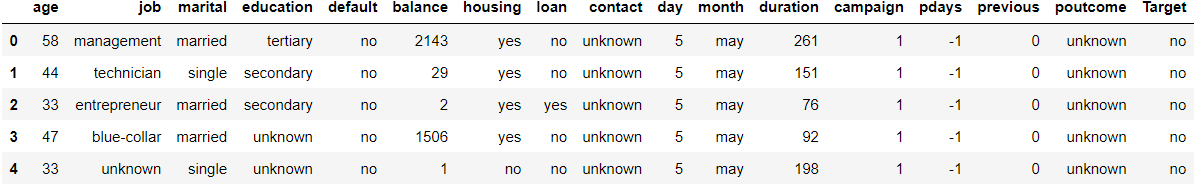
\includegraphics[width = 0.8\hsize]{./resources/img/df_head.png}
\caption{Preview of the first five rows of the dataset.} %~\cite{BBV178P113004Y2021}}
\label{fig:balance}
%\caption{Schematic diagram of Raman spectroscopy for COVID-19 detection. Schematic obtained from}
\end{figure}



\section{Objective}
In this project, our goal is to develop a predictive model for whether a client will subscribe to a term deposit or not. A \hl{term deposit is a fixed-term investment that includes the deposit of money into an account at a financial institution}. Term deposit investments usually carry short-term maturities ranging from one month to a few years and will have varying levels of required minimum deposits.
The developed model will help the bank:
\begin{itemize}
\item Understand its customers and cluster them into meaningful groups  based on their demographic and transaction information
\item Predict customer response to its telemarketing campaigns
\item Identify target customer groups for its future tele-marketing campaigns.
\end{itemize}





%    Sleek Template is a minimal collection of \LaTeX{} packages and settings that ease the writing of beautiful documents. While originally meant for theses, it is perfectly suitable for project reports, articles, syntheses, etc. -- with a few adjustments, like margins.

%    It is composed of four separate packages -- \texttt{sleek}, \texttt{sleek-title}, \texttt{sleek-theorems} and \texttt{sleek-listings} -- each of which can be used individually.

 %   \begin{lstlisting}[style=latexFrameTB, caption={Example of Sleek Template packages usage.}, gobble=8]
%        \usepackage[english]{babel}
%        \usepackage[noheader]{packages/sleek}
%        \usepackage{packages/sleek-title}
%    \end{lstlisting}

%    \blindfootnote{If you are a \LaTeX{} beginner consider the excellent \href{https://www.overleaf.com/learn}{Overleaf tutorial}. Also, there are a lot of symbols available in \LaTeX{} and, therefore, in this template. I recommend the use of \enquote{The Comprehensive \LaTeX{} Symbol List} \cite{pakin2020comprehensive} for searching symbols.}